\chapter{Software Implementation: PHD2 Guiding}
\label{ch:software-implementation-phd-guiding}

\lettrine{T}{he method} described in Chapters~\ref{ch:periodic-error-correction}
and \ref{ch:predictive-error-correction-for-telescopes} was implemented as part
of the telescope guiding software \emph{PHD2 Guiding} \cite{Stark.ea:2016:PHD2}.
PHD2 Guiding is an open-source telescope guiding software used by many amateur
astronomers. Developing the adaptive periodic error correction algorithm as a
part of PHD2 Guiding makes it possible to reach the astronomers that
already use this software. Also, by using the mature and well-engineered PHD2
Guiding platform, we do not need to take care of hardware interactions and can
instead focus on the guiding algorithm itself.

After introducing the PHD2 Guiding framework
(Section~\ref{sec:phd2-guiding-framework}), we describe several modifications
to the algorithm (Section~\ref{sec:algorithm-changes}). These changes were
necessary to increase robustness for the use by unexperienced users.
We then briefly present a guiding method for the second telescope axis
(Section~\ref{sec:the-dec-axis}) before discussing the results of experiments
with this predictive telescope guiding framework
(Section~\ref{sec:phd-guiding-experiments}).

\section{The PHD2 Guiding Framework}
\label{sec:phd2-guiding-framework}

PHD2 Guiding is a GUI-based software for telescope guiding optimized for
easy usage. Figure~\ref{fig:PHD2} shows the main window of the software with
star display and residual error curves. The software includes drivers for many
guiding cameras as well as telescope mounts, and handles the hardware
interactions. PHD2 Guiding is open-source software, so it is possible to
integrate additional features. It is under active development and is downloaded
several thousand times per month.

The current state-of-the-art guiding algorithm in PHD2 Guiding is a
proportional controller with hysteresis to prevent changes in the control
direction. This algorithm does not make use of extrapolation. The lack of a
predictive control scheme results in residual structure in the pointing error
when the sampling frequency is low. It is also not robust, \eg when a cloud
occludes the guide star for some time. In such a case the guide star is
usually lost because it moved too far away from its original position during the
period without measurements.

These two issues can be tackled with the GP framework: Structured extrapolation
together with predictive control reduces residual error and residual structure.
Also, since extrapolation and predictive control still offer a control input
even when no measurements are available, it is possible to issue control actions
in those cases. This results not only in a decrease in pointing error, but also
increases robustness because the guide star remains closer to the target
position.

\begin{figure}
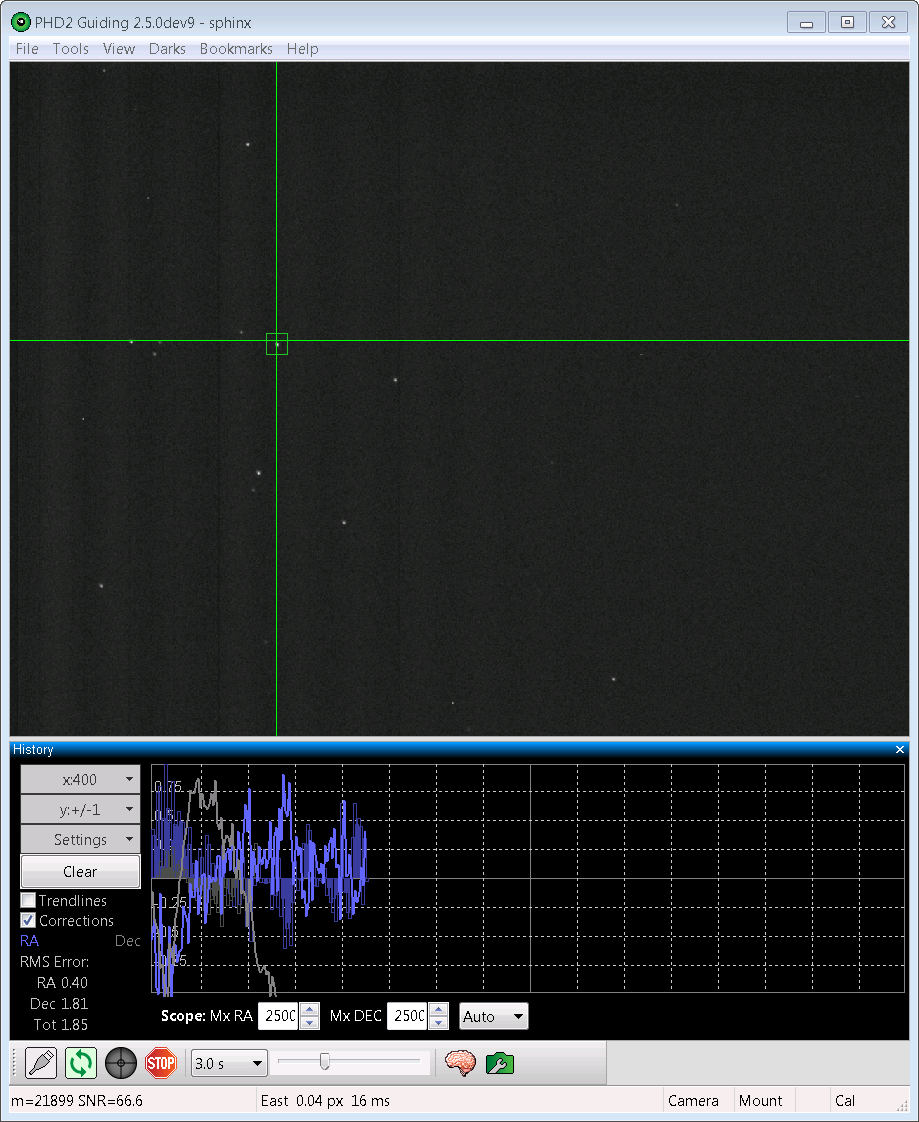
\includegraphics[width=\textwidth]{img/PHD2_screenshot_crop.png}
\caption[GUI of PHD2 Guiding in version 2.5.0.]{GUI of PHD2 Guiding in
version 2.5.0. The upper part is the star display with the guide star
highlighted by the crosshair. The search region for the guide star is the small
box. The lower part shows the residual error curves and the controls.}
\label{fig:PHD2}
\end{figure}

\section{Periodic Error Correction for PHD2 Guiding}
\label{sec:algorithm-changes}

Despite the fact that there are libraries for Gaussian processes in C++, we
chose to implement the GP algorithm ourselves. This decision was made because
some crucial features, such as the conditioning on a subset of the kernel
combination, are missing in the readily available libraries.

Much of the GP infrastructure is based on linear algebra. Thus, we selected to
use the Eigen matrix library \cite{Guennebaud.Jacobs.ea:2010:Eigen} to make
use of fast and well-tested linear algebra code. Using the Eigen library also
increases the readability of the overall implementation. The Eigen library
itself has no external dependencies and is therefore relatively easy to include
in the existing project.

\subsection{Data Acquisition}

Instead of retaining all collected data, it is necessary to limit the number
of data points to keep the computational effort bounded and the runtime
predictable. We use a FIFO buffer to store data points, where, once the buffer
is full, the oldest entry is dropped whenever a new data point is added. This
amounts to a windowing of the dataset.

Using the measured pointing error directly to identify the dynamics function
turned out to be not robust enough during our intensive testing. Therefore, we
model the \emph{accumulated} gear error
\begin{equation}
  \label{eq:accumulation-model}
 a_{k} = e_k + \sum_{i=0}^{k-1} u_i
\end{equation}
where $e_k$ is the measured pointing error at time step $k$ and $u_i$ are the
control signals at time $i$. This model is more robust because the error
introduced by the gear accumulates, while random effects caused by, \eg
the stepper motor, average out. Overall, this leads to a better
signal-to-noise ratio for the accumulated gear error compared to the absolute
pointing error.

Additionally, the measurement process does not have uniform noise. Since the
location of the guide star is determined from pixel intensities via a weighted
centroid of the star's pixels, the accuracy of the centroid calculation depends
on the signal-to-noise ratio (SNR) of the image. In PHD2 Guiding, the SNR is
calculated according to the method described by
\textcite{Simonetti:2004:Measuring}; the relation between the SNR and the
measurement noise variance was determined empirically and modeled by the linear
regression model
\begin{equation}
  \sigma(\rho) = w_{\sigma,1}(\rho - \rho_0)^{-1} + w_{\sigma,0},
\end{equation}
where $\rho$ is the SNR, $\rho_0$ is an input offset and $w_{\sigma}$ are the
parameters for the regression model. Figure~\ref{fig:snr-vs-sigma} shows this
relationship and the data used to determine it.

\begin{marginfigure}
\footnotesize
\setlength{\figurewidth}{0.8\textwidth}%
\setlength{\figureheight}{0.6\textwidth}%
\inputTikZ{snr_vs_sigma}
\caption[Relationship between the signal-to-noise ratio and measurement
variance.]{Relationship between the signal-to-noise ratio and measurement
variance. Shown are RMS errors from simulated exposures for different SNRs
(\ref*{p:snr-sig}) and the regression line (\ref*{p:snr-sig-reg}).}
\label{fig:snr-vs-sigma}
\end{marginfigure}

The value of the estimated noise variance is stored along with the measurements
of the signal. It is then used in a heteroscedastic noise model, as described in
Section~\ref{sec:heteroscedastic-noise}.

\subsection{Modeling}

\begin{figure}
\footnotesize
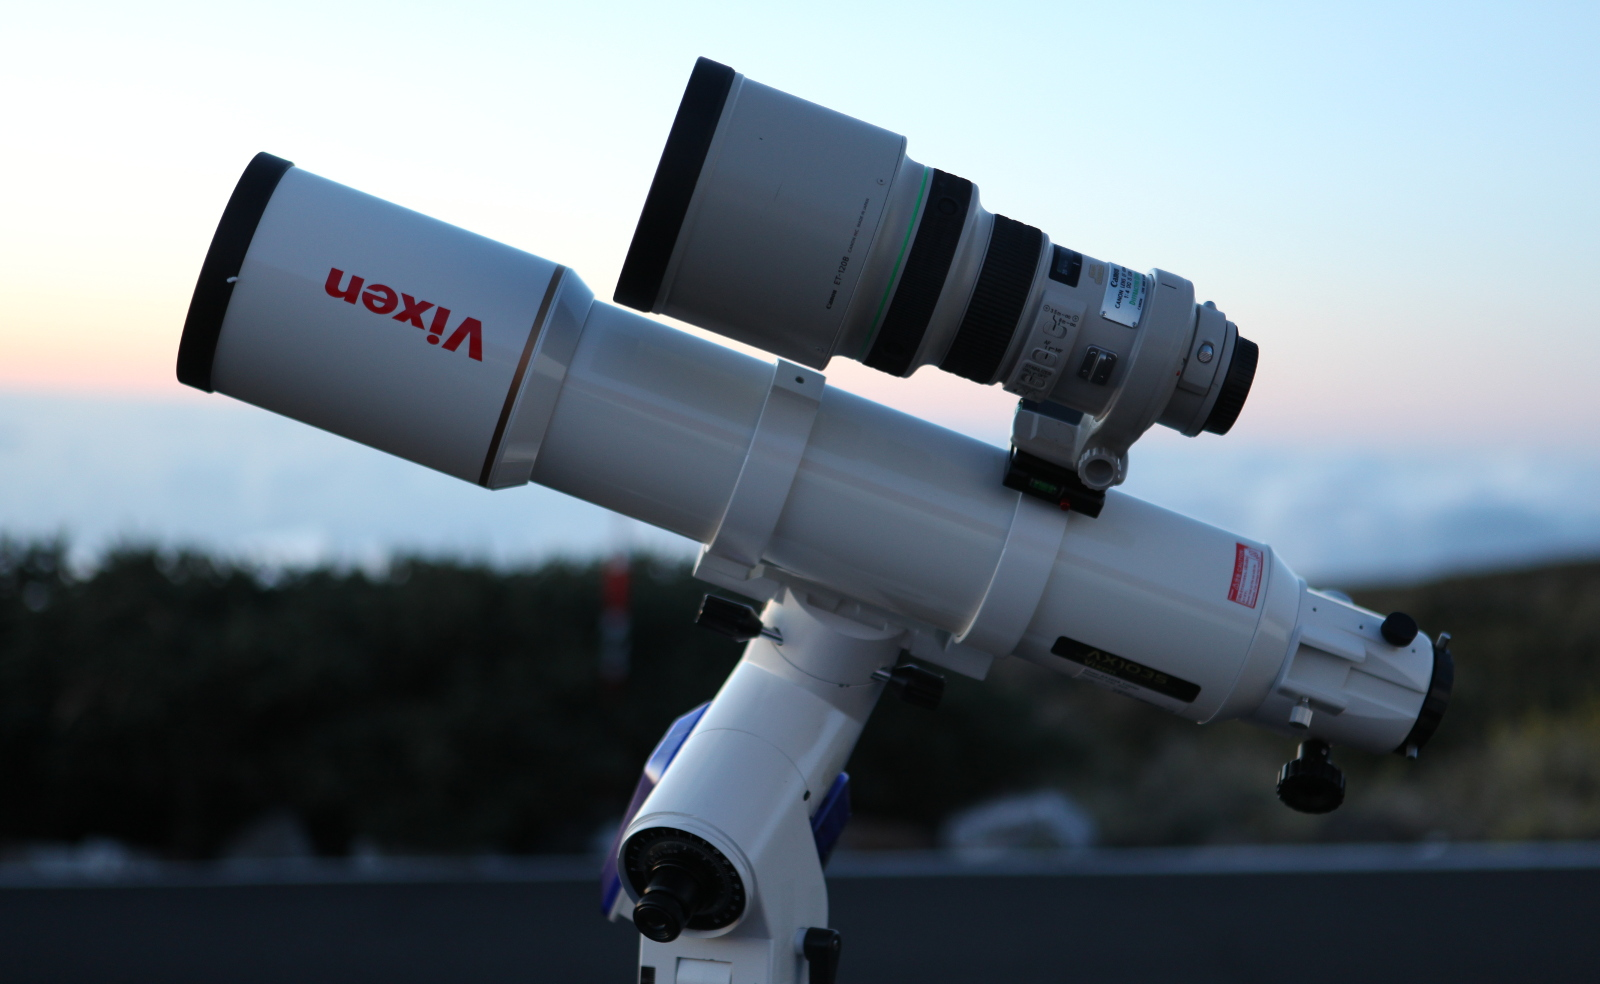
\includegraphics[width=\textwidth]{img/telescope_small.jpg}
\caption[Telescope setup with main and guiding telescope.]{Telescope setup with
main and guiding telescope. The guiding telescope is mounted ``piggyback'' on
the main imaging telescope. The cameras are not yet attached.}
\label{fig:typical-setup}
\end{figure}

In real astronomical imaging setups (see Figure~\ref{fig:typical-setup}
for an example), it is almost impossible to align the axis of the telescope
mount with the Earth's rotational axis perfectly. Thus, in most cases there will
be a moderate drift that needs to be modeled and predicted in addition to the
periodic component. As it is hard to find the linear drift component
independently of the periodic gear error, we employ a joint model as described
in Section~\ref{sec:explicit-feature-functions}, consisting of fixed features
for constant and linear components and a Gaussian process to model the nonlinear
part:
\begin{equation}
 a(t) = [\beta_0\q \beta_1]
  \begin{bmatrix}1\\t\end{bmatrix} + f(t)
\end{equation}
with $f(t)\sim\GP$. We assume an uninformative prior where $\beta\sim\N(0,B)$,
$B\inv\to 0$, as detailed in \cite[\ts2.7]{Rasmussen.Williams:2006:Gaussian}.

The GP itself consists of three different components that were identified
during experimentation. It is also possible to automatically identify kernel
components \cite{Duvenaud.Lloyd.ea:2013:Structure}, but for this application
the hand-crafted kernels were more compact and robust. The different components
are:
\begin{description}
  \item[slowly-varying SE] Not all mechanical effects are periodic.
    In order to allow for mechanical deviations, \eg deformations due to load
    shift in the mechanics, we include a long-length-scale square exponential
    kernel. As a result of the long length scale, this part of the model is
    also amenable to extrapolation.
    \begin{equation}
      \k_{\mathsc{se},0}(t, t'; \theta_0, \ell_0) = \theta^2_0
      \exp\left(- \frac{|t-t'|^2}{2\ell^2_0}\right)
    \end{equation}
  \item[periodic] The periodic component is the important part of the model. It
    captures the recurrent disturbances from the gear. This component was chosen
    to be periodic to enable long-term predictions.
    \begin{equation}
      \k_\mathsc{p}(t,t';\theta_\mathsc{p},\ell_\mathsc{p},\lambda) =
      \theta^2_\mathsc{p}
      \exp\left(-\frac{2\sin^2\left(\frac{\pi}{\lambda}
      (t-t')\right)}{\ell^2_\mathsc{p}}\right)
    \end{equation}
  \item[quickly-varying SE] Since the actual data is not perfectly periodic, we
    allow for fast variations with a square exponential kernel with short
    length-scale. This kernel captures deviations due to mechanical
    roughness.
    \begin{equation}
      \k_{\mathsc{se},1}(t, t'; \theta_1, \ell_1) = \theta^2_1
      \exp\left(-\frac{|t-t'|^2}{2\ell^2_1}\right)
    \end{equation}
\end{description}

The combined kernel function is the sum of the three individual kernel functions
\begin{fullwidth}\vspace{-\baselineskip}
\begin{equation}
  \label{eq:compund-kernel}
  \k_\mathsc{c}(t,t';\boldsymbol{\eta}) =
\k_{\mathsc{se},0}(t,t';\theta_0,\ell_0) +
\k_\mathsc{p}(t,t';\theta_\mathsc{p},\ell_\mathsc{p},\lambda) +
\k_{\mathsc{se},1}(t,t';\theta_1,\ell_1),
\end{equation}
\end{fullwidth}
where we have subsumed parameter dependencies into the parameter vector
$\boldsymbol{\eta}=[\theta_0, \ell_0, \theta_\mathsc{p},\ell_\mathsc{p},
\lambda, \theta_1, \ell_1]$.
A sample from the compound model, combining the linear part and the GP with
kernel function \eqref{eq:compund-kernel} is shown in
Figure~\ref{fig:model-components}.

\begin{figure}
\footnotesize%
\setlength{\figurewidth}{\textwidth}%
\setlength{\figureheight}{0.6\textwidth}%
\inputTikZ{model_components}%
\caption[Combining the components of the model.]{Combining the components
of the model: Linear drift (\ref*{p:mod-lin}), plus long
length-scale SE (\ref*{p:mod-se}), plus periodic (\ref*{p:mod-se-per}), plus
short length-scale SE (\ref*{p:mod-se-per-se}). One sample of the model is
generated from the individual components.}
\label{fig:model-components}
\end{figure}

The overall model is expressive enough to capture the different aspects of
the problem. While linear drift, slowly-varying SE and the periodic
component are features that can be extrapolated, the quickly-varying SE can not.
It regresses back to the mean quickly after the last data point,
which disturbs the controller. Therefore, while inference is done with the
full model, the predictions are conditioned on the model without the
quickly-varying SE. See Section~\ref{sec:output-projections} for the
details on the output conditioning.

\subsection{Hyperparameter Identification}

While many of the hyperparameters included in the model can be estimated by
mechanical considerations without affecting performance too much, one
parameter can not: the period length $\lambda$. It is crucial for the predictive
power that this parameter closely matches the mechanical period length; there
is little robustness regarding the choice of this parameter.

Instead of relying on the maximization of a probabilistic criterion, the
identification of the main periodic component is done with classic spectrum
analysis. After subtraction of a polynomial fit of order 1 to remove the linear
trend, a Hamming window \cite[\ts7.2.1]{Oppenheim.ea:1999:Discrete} is applied
to reduce spectral leakage effects due to the finite-length signal.

In order to obtain the spectral density of the measured signal, the discrete
Fourier transform (DFT) \citenum[\ts8.1]{Oppenheim.ea:1999:Discrete} is
calculated on the preprocessed data
\begin{equation}
  \label{eq:DFT}
  s_k = \sum_{n=0}^{N-1} a_n e^{-\frac{2\pi \imath}{N} nk},
\end{equation}
where $\mathbf{s}=[s_0, \dots, s_{N-1}]$ is the spectrum, $\mathbf{a}=[a_0,
\dots, a_{N-1}]$ is the data and $\imath$ is the imaginary unit. The period
length of the strongest frequency component is subsequently calculated from the
power spectrum $\mathbf{s}$. In order to ensure constant frequency resolution,
the data vector is zero-padded up to the maximum number of data points in the
FIFO buffer.

In the software implementation, we use the fast Fourier transform (FFT)
\margincite{Gauss:1866:Theoria}\margincite{Cooley.Tukey:1965:Algorithm}
\citenum{ Gauss:1866:Theoria, Cooley.Tukey:1965:Algorithm}
for the spectrum analysis, since the na{\"i}ve
implementation of \eqref{eq:DFT} is not viable for the online use.

\subsection{GP Approximation}

It is important to note that in the case of periodic covariance functions, it
is not enough to do a simple windowing because it is necessary to cover
multiple periods with the data for decent predictive performance. Depending on
the choice of sampling frequency, it is often too expensive to use a full
dataset of consecutive measurements to cover multiple periods. Instead, the
FIFO buffer holds multiple periods worth of measurements and we use a
subset-of-data (SD) approximation to keep inference cheap. See
Section~\ref{sec:subset-of-data} for the details of the SD method.

The fact that the extrapolation position is known in advance is beneficial in
this case. In order to obtain a computationally cheap method, we use the
covariance between the prediction point and the data to select the data points
for the approximation:
\begin{equation}
  \mathbf{x}_\mathsc{sd} = \mathtt{sort}\left\{\mathbf{x}; \k(
\mathbf{x},x)\right\}_{0:M-1},
\end{equation}
where $\mathbf{x}_\mathsc{sd}$ is the selected dataset, $\mathtt{sort}$ sorts
the data $\mathbf{x}$ according to the values of the covariance vector $\k(
\mathbf{x},x)$ and $\{\cdot\}_{0:M-1}$ selects the first $M$ elements.

For each control step, we select a new subset from the large dataset in the FIFO
buffer, depending on the current prediction point. This way we make sure that
there is always relevant data from past periods available to the GP, while
keeping the inference cost low.

\subsection{Control}

The control algorithm used in the guiding software was designed to avoid the
problems that arise from the low sampling frequency, while keeping the
complexity of the algorithm low. Ideally, one would implement an optimal
control scheme as introduced in Section~\ref{sec:control}, but for the
simplicity of the algorithm, only a ``deadbeat'' controller\footnote{A deadbeat
controller is a predictive controller that is tuned to eliminate the entire
error in one step, \ie the error-feedback gain is 1.} was considered. Due to
the low sampling frequency and non-uniform sampling intervals, this deadbeat
control often led to overshoots and instabilities. Reducing the control gain, on
the other hand, led to performance loss due to the periodic error.

The implemented algorithm, therefore, is a hybrid controller: Deadbeat control
is applied for the compensation of the periodic error, and proportional control
is used to drive the residual error to zero. The overall control signal at time
$k$ is given by
\begin{equation}
  \label{eq:dead-P}
  u_k = -(\tilde a_{k+1} - \tilde a_{k}) - g_\mathsc{p} e_k,
\end{equation}
where $\tilde a_{k}$ is the mean prediction of the Gaussian process
modeling the accumulated gear error $a_k$, and $g_\mathsc{p}$ is the control
gain for the proportional controller. The structure of this
hybrid control algorithm is shown in Figure~\ref{fig:PEC_controller}.

\begin{figure}%
  \center%
  \inputTikZ{PEC_controller}%
  \caption[Structure of the telescope controller for the RA axis.]{
Structure of the telescope controller for the RA axis. While the residual error
is handled with proportional control, the GP prediction is accounted for in a
deadbeat fashion.}
  \label{fig:PEC_controller}
\end{figure}

\section{The Declination Axis}
\label{sec:the-dec-axis}

When the alignment between the right ascension (RA) axis and the Earth's
rotational axis is not perfect, the offset introduces a linear drift in the
image plane for \emph{both} axes. Therefore, also the declination (Dec) axis
needs to be controlled.

However, since the declination axis is almost still and only needs to
compensate small drift errors, the regression problem is different from the RA
axis: Due to the low signal-to-noise ratio and the small drift, the control
signal of a proportional control often changes its sign. This leads to gear
backlash effects, disrupting even usual robust regression models, such as
$\ell_1$-regression or Huber-regression \cite{Huber:1964:Robust}.

Since the underlying dynamical model is simple, and the estimation only needs to
find a linear drift, we implemented a trimmed mean estimator for the linear
drift:
\begin{equation}
  \Delta \tilde a^\text{Dec}_{k+1} = \frac{1}{k-2n_T}
    \sum_{i=n_T}^{k-n_T-1} \mathtt{sort}\left\{\mathbf{\Delta
a}^\text{Dec}_{1:k}
  \right\}_i,
\end{equation}
where $\mathbf{\Delta a}_{1:k}^\text{Dec}$ is the collection of finite
differences of the accumulated gear errors $a_k^\text{Dec}$ and $n_T$ is the
number of elements to trim on either side. The $\mathtt{sort}$-operator sorts
the collection according to the values, and $\{\cdot\}_i$ selects the $i$-th
element.

The control structure, which is similar to \eqref{eq:dead-P}, is
shown in Figure~\ref{fig:TM_controller}. The estimated drift
$\Delta \tilde a^\text{Dec}_{k+1}$ is corrected for in a deadbeat
fashion, while the error term is driven to zero with a conservatively-tuned PD
controller \cite{Astrom.Hagglund:1995:Theory}.

\begin{figure}%
  \center%
  \inputTikZ{TM_controller}%
  \caption[Structure of the telescope controller for the Dec axis.]{
Structure of the telescope controller for the Dec axis. While the residual error
is handled with PD control, the prediction from a trimmed-mean estimator is
accounted for in a deadbeat fashion.}
  \label{fig:TM_controller}
\end{figure}

\section{Experiments}
\label{sec:phd-guiding-experiments}

The demonstration of the implemented guiding algorithm was done for the
use-case of tracking stars in the night sky (as opposed to the laboratory setup
of Section~\ref{sec:hardware}). The measurements were made in T{\"u}bingen,
Germany, using a \emph{Vixen} Sphinx telescope mount with a \emph{Canon} EF 400
DO IS USM lens and a \emph{The Imaging Source} DMK 41AU02.AS camera, the same
equipment as in the laboratory setup.

\subsection{Guiding Performance}

The performance of GP guiding is shown in comparison to the state-of-the-art
algorithm\footnote{In PHD2 Guiding, the standard algorithm is ``Hysteresis'',
which is a P-controller with hysteresis to prevent gear backlash effects.} that
is used in PHD2 guiding. Figure~\ref{fig:comparison-sota} shows the exemplary
comparison of the two algorithms under otherwise identical conditions. The
angular pointing error between target position of a guide star and its measured
position is plotted over time. It is visible that the GP guiding shows less
residual structure after the initial learning phase (up to around
1000\unit{s}). Since the GP guider starts with zero information, the effect of
learning is visible in the data by the structural change in the error residuals
after 1000\unit{s}.

\begin{figure}
\setlength{\figurewidth}{0.95\textwidth}%
\setlength{\figureheight}{0.4\textwidth}%
\footnotesize
\inputTikZ{comparison_sota}
\caption[Comparison between state-of-the-art tracking
and GP-based tracking.]{Comparison between state-of-the-art tracking
of PHD2 Guiding 2.5.0 (top, \refpoints{p:comp-sota}) and GP-based tracking
(bottom, \refpoints{p:comp-gpg}).}
\label{fig:comparison-sota}
\end{figure}

When analyzing the guiding performance, the initial learning phase has to be
compared separately. We report the mean, standard deviation and RMS error of the
two different algorithms for the different phases. The GP guiding consistently
outperforms the standard algorithm.

\begin{table}[ht]
{\centering
\footnotesize
    \begin{tabular}{l|rrr|rrr|rrr|}
    & \multicolumn{3}{c|}{overall} & \multicolumn{3}{c|}{for $t<1000$} &
      \multicolumn{3}{c|}{for $t>1000$}\\
    & mean & \mathsc{sd} & \mathsc{rms} & mean & \mathsc{sd} & \mathsc{rms} &
      mean & \mathsc{sd} & \mathsc{rms}\\
    \midrule
Hy & 0.357 & 0.968 & 1.031 & 0.427 & 0.917 & 1.010 & 0.331 & 0.985 &
1.039 \\
GP & 0.122 & 0.751 & 0.761 & 0.088 & 0.893 & 0.895 & 0.136 & 0.685 &
0.697 \\
  \end{tabular}
\vskip 0.1in
\caption[Experimental results from outdoor telescope tracking.]{Experimental
results from outdoor telescope tracking (all numbers
in \as). ``Hy'' is the standard ``Hysteresis'' algorithm and ``GP'' is
the GP guiding algorithm developed in this thesis. In addition to the overall
performance, we report the performance for the initial phase ($t<1000$) and for
the later phase ($t>1000$) separately.}
\label{tab:results-stars}
}
\end{table}

\subsection{Dark Guiding}

In order to show the improved robustness under conditions where the measurement
is unavailable for some time, we implemented a dark guiding mode. When there is
no measurement, the guiding is done with the GP predictions alone. This prevents
the telescope from moving away from the guide star too quickly, increasing
chances of finding the guide star after recovery of the measurement process.

Figure~\ref{fig:cloud-tracking} shows the benefit of the GP guider under
occlusion conditions. With the GP guider the linear and periodic motion is
predicted, keeping the pointing error comparably small. The state-of-the-art
algorithm does not predict the motion of the telescope, leading to larger
pointing errors after an occlusion period.

\begin{figure}
\setlength{\figurewidth}{0.95\textwidth}%
\setlength{\figureheight}{0.5\textwidth}%
\footnotesize
\inputTikZ{cloud_tracking}
\caption[Tracking under cloudy conditions.]{Tracking under cloudy conditions.
After enough time for learning, the measurements were dropped for a few minutes,
simulating the effect of a cloud covering the guide star. The plot shows the
accumulated gear error $a_{k}$ from measurements (\refpoints{p:cloud-gear}), and
the predictive mean (\ref*{p:cloud-prediction}) and uncertainty
(\ref*{p:cloud-unc}) for the time without measurement (indicated by
\ref*{p:cloud-dark}). The ``prediction'' of the state-of-the-art algorithm is
flat (\ref*{p:cloud-flat}).}
\label{fig:cloud-tracking}
\end{figure}

\section{Conclusion}

Making the Gaussian process based periodic error correction algorithm available
to many practitioners in astrophotography was an important goal of this
project. In order to make the algorithm work on a broad range of telescopes,
a number of changes to the algorithm were developed and implemented, such as a
hybrid control strategy and the parameter identification via FFT.

In experiments under realistic conditions we showed that the implemented
algorithm provides improved tracking performance and can even deal with the
case of an unreliable measurement process due to clouds.
